\documentclass[Main]{subfiles}
\begin{document}

\chapter{Mathematical Preliminaries}
%Intro
%-_-_-_-_-_-_-_-_-_-_-_-_-_-_-_-_-_-_-_-_-_-_-_-_-_-_-_-_-_-_-_-_-_-_-_-_-_-_-_-_-_-_-_-_-_-_-_-_-_-_-_-_-_-_-_

	\begin{Warning}
		Le interazioni matematiche sono complesse  e non triviali (vedi un po' di articoli di introduzione a AQFT per ispirarti)
		
		Tendenzialmente le teorie quantistiche di campi moderne sono di Quantizzazione.. Quindi richiedono di specificare bene la struttura del campo classico (vedi intro di Mangiaratti shardashivly)
		
		Gli strumenti matematici per raccontare la teoria dei campi classici sono essenzialmente 3: Fibrati, S-T G-H, LDOP e GHOP.
		
		IN questo paper non ci soffermeremo sulle strutture del framework puramente quantistico (* algebre e quant'altro). Per un primer vedere articolo di Dappiaggi o Libro Adv aqft.
		
		Diamo per scontato un background di base in Geometria differenziale e derivate esterne (algebre di Grassman? global calculus? non so come chiamarlo!).
		
		Potrei avere la tentazione a provare ad usare un po' di linguaggio basilare delle categorie... la mia fonte è \href{http://katmat.math.uni-bremen.de/acc/acc.pdf}{Joy of Cat}.
	\end{Warning}
	
	\begin{Warning}
		Stile: Intro lapiadaria ai 3 argomenti ( bundle cinematica di campo, Glob iper stage per descrivere dinamica di tipo propagativo, Operatori tipo onda). Poi smitragliata di definizioni come faceva Penati.
	\end{Warning}	


%-_-_-_-_-_-_-_-_-_-_-_-_-_-_-_-_-_-_-_-_-_-_-_-_-_-_-_-_-_-_-_-_-_-_-_-_-_-_-_-_-_-_-_-_-_-_-_-_-_-_-_-_-_-_-_
%-_-_-_-_-_-_-_-_-_-_-_-_-_-_-_-_-_-_-_-_-_-_-_-_-_-_-_-_-_-_-_-_-_-_-_-_-_-_-_-_-_-_-_-_-_-_-_-_-_-_-_-_-_-_-_
	\section{Fiber Bundles}
		\danger intro
		
		\subsection{Formal Definition}
			Although it would be possible to present the concept \emph{bundle} in a more general way through the language of categories, for our argument will be sufficient to consider only the case of \emph{smooth bundles}.

			\begin{definition}[Fiber Bundle]\label{Def:SmoothBundle}
				A \emph{Fiber Bundle} consists in a 4-ple $(E,M,Q,\pi)$ where:
				\begin{itemize}
					\item[-] $E,M,Q$ :  smooth manifolds called respectively \emph{Total Space}, \emph{Base Space}, \emph{Typical Fiber}.
					\item[-] $\pi : E \rightarrow M $ continuous smooth function (called \emph{Bundle Projection})
				\end{itemize}
				Endowed with a \emph{Local Trivialization}:
				\begin{itemize}
					\item $\forall x \in E$ $\exists$ a couple $(U, \chi)$ (called \emph{local trivialization})
					\begin{itemize}
						\item $U$ : neighborhood of $x$
						\item $\chi$ :$\pi^{-1}(U) \rightarrow U \times Q$ : diffeomorphism
							%DaRivedere
 							\footnote{surjectivity $\Rightarrow$ $\pi^{-1}(U) \neq \emptyset$.} 
 							\footnote{cartesian product of topological space is a topological space with the direct product topology.}
					\end{itemize}
					such that: $p_1 \cdot \chi = \pi \vert_{\pi^{-1}(p)}$.

					i.e: the following graph commutes:
					\begin{tikzpicture}
						 \matrix (m) [matrix of math nodes,row sep=3em,column sep=4em,minimum width=2em] {
     						\pi^{-1}(U) & U \times Q \\
     						U &  \\};
 						 \path[-stealth]
 							(m-1-1) edge node [left] {$\pi$} (m-2-1)
            				edge [right] node [above] {$\chi$} (m-1-2)
    						(m-1-2) edge [right] node [below] {$p_{1}$} (m-2-1);;
					\end{tikzpicture}

				\end{itemize}
			\end{definition}

			\begin{figure}[h!]
  				\caption{The complete fiber bundle Structure.}
  				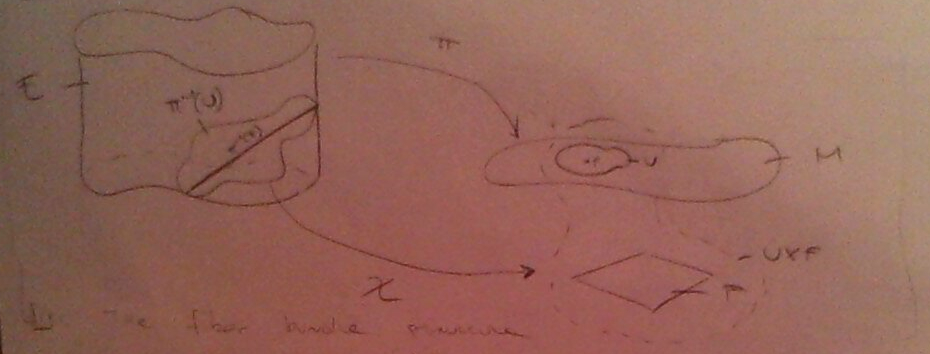
\includegraphics[width=0.5\textwidth]{Pictures/FiberBundle}
  				\centering
			\end{figure}
			\begin{notationfix}
				It is customary to refer to a vector bundle specifying only its total space:
				\begin{displaymath}
					\gls{Bundle}%E= ( E,\pi, B ; F)
				\end{displaymath}
			 	In the following we adopt this convention whenever this does not lead to misunderstandings.
			\end{notationfix}
			
			\begin{observation}
				For all $p\in M$ we refer to the submanifold $E_{p} := \pi_{-1}(p) \subset E $ as \emph{fiber over the point p}.
				\\
				Every fiber $E_p$ is diffeomorphic to the typical fiber $F$ through the local trivialization charts.
			\end{observation}
			
			\begin{notationfix}
				We say that a smooth bundle E is \emph{(globally) trivial} if $E \simeq M \times Q$ i.e there exists a trivialization of $E$ which is defined everywhere.
				Note that definition \ref{Def:SmoothBundle}  prescribes the existence of local trivializations only.
			\end{notationfix}
			
			When a smooth fiber bundle $(E,\pi,M;Q)$ is considered, in addition to the typical functions of the bundle $(\pi, \chi_{\alpha})$ should be taken in account also  the local charts $(U_{\alpha_k}, \phi_{\alpha_k})_{k = E,M,Q}$ provided by the atlases of $E,M$ and $Q$:
			\begin{definition}[Bundle atlas]
				Collection local chart which trivializes $E$. I.e. triples  $(U_\alpha, \psi_\alpha, \chi_\alpha)$ where:
				\begin{itemize}
					\item $U_\alpha$ open set in $M$ such that $\bigcup_{\alpha} U_{\alpha} \supseteq M$.
					\item $\chi_\alpha$  is a local trivialization.
					\item $(U_\alpha,\psi_\alpha)$ local chart on $E$ constructed from charts on the base and fiber manifold:
						\begin{displaymath}
							\psi^{(E)}_\alpha = \psi_\alpha^{(M)} \times  \psi_\alpha^{(Q)} \circ \chi_\alpha
						\end{displaymath}	
				\end{itemize}		
			\end{definition}
			
			
						
			Endowing the bundles manifolds with other additional structures, can be introduced important subclasses of smooth bundles:
			\begin{definition}[Vector Bundle]
				Is a smooth bundle $E=(E,\pi,M;V)$ such that:
				\begin{itemize}
					\item The typical fiber manifold $V$ is a finite dimensional vector space.	
					\item All the trivialization $\chi_{\alpha} $ are diffeomorphism such that:
						\begin{displaymath}
							\chi_{\alpha}\vert_{\pi^{-1}(p)} \in \mathbb{GL}(n, \mathbb{R})
						\end{displaymath}
				\end{itemize}
			\end{definition}

		\subsection{Cross Sections}
			The notion of bundle is particularly interesting from the perspective of physics because provides the rigorous description of a $Q-$valued field over the space $M$:			
			\begin{definition}[Smooth Section]
				Function $\phi : M \rightarrow E$ such that:
					\begin{itemize}
						\item $\phi$ smooth.
						\item $\phi \cdot \pi = \Id_M$ 
					\end{itemize}
			\end{definition}
			
			\begin{notationfix}
				We refer to:
					\begin{itemize}
						\item \emph{Global section} $\Leftrightarrow$ $\textrm{dom}(\phi) = B$
						\item \emph{Local section} $\Leftrightarrow$ $\textrm{dom}(\phi) \subset B$ \footnote{Usually the domain is an open set of B)}
					\end{itemize}
				We denote the set of all the smooth sections of the bundle $E$  as:
				\begin{displaymath}
					\gls{Sections}
				\end{displaymath}
			\end{notationfix}
			
			\begin{observation}
				\gls{Sections} is an infinite dimensional manifolds.	
			\end{observation}
			If $E$ is a vector bundle \gls{Sections} is an infinite dimensional vector space, therefore we can introduce the  on a base:
			
		\subsection{Mapping between Bundles}
			%Bundle morphism
			
			%mor bundle
			
			%pullback bundle
			
					
					

			
			
		\subsection{Tangent Bundles}
			\subsubsection{Tautological one-form and simplectic form.}
				Fomm: As a mathematical curiosity, we note that the cotangent bundle of any
manifold is orientable. Indeed, it carries a symplectic structure and hence a volume element.			
					
		\subsection{Jet Bundles}
			$\Obj (A)$			
			$\hom(A,B)$
			$\Mor$
			$\cod \dom \ran$
%-_-_-_-_-_-_-_-_-_-_-_-_-_-_-_-_-_-_-_-_-_-_-_-_-_-_-_-_-_-_-_-_-_-_-_-_-_-_-_-_-_-_-_-_-_-_-_-_-_-_-_-_-_-_-_
%-_-_-_-_-_-_-_-_-_-_-_-_-_-_-_-_-_-_-_-_-_-_-_-_-_-_-_-_-_-_-_-_-_-_-_-_-_-_-_-_-_-_-_-_-_-_-_-_-_-_-_-_-_-_-_
	\section{Globally Hyperbolic Space-times}
			\begin{Warning}
				Mettere solo le definizioni che uso prese dagli articoli di review delle Fonti
			\end{Warning}	
			Appunti che mi ero preso scrivendo il secono capitolo:
					
			This condition is strictly connected to the dynamic behaviour of the system.
			
			\begin{Warning}
			Def di dominio di dipendendenza
			footnote di definizione di spazio tempo
			def cauchy surface
			Remark causal future past
			def globally hyperbolic
			Teorema sulle caratterizzazioni
			\end{Warning}			
			
			\begin{notationfix}
				We denote the set of all the cauchy surfaces as $\PowerSet_{C}(M)$.
			\end{notationfix}
					

		Glon iperbolic determina la fogliazione dello spazio tempo per superfici di cauchy
		La superficie di cauchy è questa:
		\begin{definition}[Cauchy surface]
		\end{definition}		
		questo da la possibilità della buona posizione dei problemi di cauchy.. fisicamente è la condizione minima per definire i dati iniziali dell'evoluzione dinamica.
		definisco data...
						
		\begin{Warning}
		Rapporto con la condizione sugli operatori...		
		
				
	No!		La definizione di green hyperbolicity non garantisce invece l'esistenza e unicità del problema di cauchy associata
		
		e non solo, anche l'esistenza degli operatori di green associati che sono ingrediente fondamentale della costruzione di peierls

		M è glob iper e P è green iper per tener conto del comporatamento propagativo
		definire sup cauchy
		definire s-t iperbolico (solo la caratterizzazione di ammetre una sup di cauchy)
		definire op green iperbolico su spazio tempo iperbolico (cioè ha delle green ope)
		Propr di buona definizione esistenza e unicita della soluzione
		
		Di particolare ricorrenza fisica sono gli operatori normally iperbolic
		espressione in coordinate
		esempio K-g!
		\end{Warning}						
		
		\begin{Warning}
			Far notare che minkowski e tanti esempi importanti sono GH
		\end{Warning}
		
		\begin{observation}
		(che serve dopo) lo spazio $R$ è banalmente iperbolico in quanto tutti i punti posso essere visti come superfici di cauchy.
		\end{observation}
			
					\subfile{DefinitionBulk2}		


%-_-_-_-_-_-_-_-_-_-_-_-_-_-_-_-_-_-_-_-_-_-_-_-_-_-_-_-_-_-_-_-_-_-_-_-_-_-_-_-_-_-_-_-_-_-_-_-_-_-_-_-_-_-_-_
%-_-_-_-_-_-_-_-_-_-_-_-_-_-_-_-_-_-_-_-_-_-_-_-_-_-_-_-_-_-_-_-_-_-_-_-_-_-_-_-_-_-_-_-_-_-_-_-_-_-_-_-_-_-_-_
		\section{Green Hyperbolic Operators}
			\begin{Warning}
				Mettere solo le definizioni che uso prese dagli articoli di review delle Fonti
		\end{Warning}	
					\begin{Warning}
				Pensavo di utilizzare la definizione di Green hyperbolic data da Bar che si avvale del concetto di formally dual (che non richiede la presenza del pairing) invece di quella usata in Advances AQFT che richiede solo che ammetta almeno un $G^\pm$  per poi dimostrare tramite teorema che se è anche autoaggiunto vale l'unicità. Si tratta solo di una piccola sfumatura.. Deve essere chiarito che in tutto ciò che faccio interessano che $$\forall P \, \exists1!G^\pm$$.
				Che poi questa condizione derivi da GH secondo bar o Gh secondo dap+selfadj è una di quelle questioni propriamente matematiche che poco interessa ai fisici della commissione.
			\end{Warning}			
			
			\begin{Warning}
			Devo richiedere che il green operator sia unico? sia negli schemi di quantizzazione che nella definizione di peierls faccio largo uso dell'unicità. 
			Per provare questa unicità si passa per la definizione di una forma bilineare che permette di parlare di aggiunto formale e quindi avvalersi del teorema.
			\end{Warning}
			
		    Green-hyperbolic operators are not necessarily hyperbolic in any PDE-sense and that they cannot be characterized in general by well-posedness of a Cauchy problem. \cite{Terlaky2010} \cite{Bar2010}
		
		
		
				\subfile{DefinitionBulk3}
				

\end{document}